

\chapter{``Vanilla'' Tao}
\label{c:vanilla_tao}

%----------------------------------------------------------------
\section{Before we start...}
\label{s:before_beginning}

\tao is readily customizable. All the bookkeeping is taken care of
automatically and all you need to do custom analysis is write the
subroutines pertinent to your project. However beginners are advised
to start with ``out of the box'' \tao while getting to know the
program. This tutorial starts here and will then show you how to
customize \tao for your specific purposes.

\subsection{Getting and Compiling Tao}
\index{Compiling Tao}
\label{s:get_and_compile}

The following instructions are for Cornell people. If you are not at
Cornell then the source files can be obtained at:
\begin{example}
  http://www.lepp.cornell.edu/bmad
\end{example}

In any case help may be obtained by contacting David Sagan
\cmd{<dcs16@cornell.edu>} or Jeff Smith \cmd{<js344@cornell.edu>}.

Before running \tao at Cornell the appropriate environmental variables
must be set. The way \tao is developed is that the source code is kept
in a central ``repository'' which is controlled by a software package
called \vn{CVS}. Every so often (typically about once a week) a copy
of the source code in the repository is made and a version of \tao is
compiled from this copy. This is called a ``release''. There are two
major releases: One called ``devel'' is made from the very latest
code. There is also a ``current'' release which comes from older
code. The general idea is that devel should have the latest stuff but
current should be more stable (have less bugs). In practice, since
\tao is new and the bugs are still being worked out, the devel release
is typically less buggy and hence is devel is what is recommended. To
set the environmental variables to point to the devel release do the
following.  If you are using the bash shell put the following in your
\vn{.login} file:
\begin{example}
  CESRLIB=devel
  . /home/cesrulib/bin/cesrdefs
\end{example}
If you are using tcsh put in your \vn{.login} file: 
\begin{example} 
  setenv CESRLIB devel
  source /home/cesrulib/bin/cesrdef
\end{example}
This sets the appropriate environmental variables to point to the
``devel'' ``release

After setting up the environmental variables \tao is run with the command
\begin{example}
  \$CESR_EXE/tao
\end{example}
If there has been a bug fix that you need which is in the CVS
repository but not yet in the devel release, you need to create and
use a local copy of \tao. To checkout a copy of \tao from the CVS
repository use the command \cmd{'cesrcvs co tao'} in the directory
from where you want to run \tao, (hereto referred to as
\vn{ROOT}). The checked out copy of \tao will be put in a directory
\cs{ROOT/tao}. Basically the only time a local copy of \tao is needed
is when there have been changes made to CVS that are needed that
haven't found their way to the released version. Once you have created
a local copy of \tao you may need to update it from time to time when
changes to the repository have been made by the maintainers of
\tao. To do this use the command \cmd{'cesrcvs update'} in the
\cs{ROOT/tao} directory. Note: Unless you are a maintainer, you do not
have privileges to modify the repository.



If you already have a
local copy of \tao and want to update

From the newly created \cs{ROOT/tao} directory type `\cmd{gmake}' to
create the libraries and then type `\cmd{gmake -f M.tao}' to create
the ``vanilla'' \tao program. Vanilla \tao is the basic \tao program
without any user customizations. If you are using a custom version of
\tao then follow the compiling directions from the custom \tao
author. Keep in mind that command syntax and usage may vary between
custom versions of \tao (this is a \textit{feature}, \textbf{not} a
bug!).

Once \tao has compiled go to the subdirectory \cs{ROOT/tao/program}
and type \cmd{../../bin/tao} to run ``vanilla'' \tao. This directory
contains all the configuration files to get everything working. The
first time you run the program it will need to create a digested \bmad
lattice file for the included lattice. This may take a few minutes.

\subsection{Customizing Tao}
\index{customizing Tao}

After you are familiar with the basics of \tao you are ready to fully
exploit the versatility of this wonderful program. See
Chapter~\ref{c:custom_tao} to learn how to do this. But here we will
first explore the basic functionality of the program.

%----------------------------------------------------------------
%----------------------------------------------------------------
\section{In the Beginning...}
\label{s:beginning}

%----------------------------------------------------------------
\subsection{there was the user.}

This tutorial assumes you are already familiar with basic particle
beam dynamics and its formalism. There are several books that
introduce the topics very well. The best the author has found so far
is \textit{The Physics of Particle Accelerators} by Klaus Wille.

\tao is based on the \bmad subroutine library and you should have a
working knowledge of the conventions used by \bmad. \tao can be used
``out of the box'' so an understanding of the nitty-gritty details of
\bmad is not necessary, however, one should be familiar with the
material in Part I of the \bmad manual. This part will also summarize
the particle beam dynamics used by \tao.

So, what's \tao good for? A large variety of applications. It's
versatility is that it's easily expandable. Think of it as an
accelerator design and analysis environment. The entire \bmad library
is at your disposal. But even without any customizations \tao will do
much analysis. These problems fall into three main categories:

\begin{itemize}
\item 
Design a lattice subject to various constraints.
\item
Simulate errors and changes in machine parameters. For example, you want to
simulate what happens to the orbit, beta function, etc., when you change
something in the machine. 
\item 
Simulate machine commissioning including simulating data measurement and
correction. For example, you want to know what steering strength changes will
make an orbit flat.
\end{itemize}

Programs that are written to solve these types of problems have common
elements: You have variables you want to vary in your model of your
machine, you have "data" that you want to view, and, in the first two
categories above, you want to match the machine model to the data (in
designing a lattice the constraints correspond to the data).

This tutorial is designed to informally get you, the user, up and
running with \tao without needing to dredge through the entire
reference manual. Full command syntax or greater detail on any topic
can be found in Part~\ref{ref_guide} and above.

%----------------------------------------------------------------
\subsection{Then there was the Super-universe.}\index{Super-universe}

Everything known to \tao is placed in an area called the
\textit{super-universe}. Within the \textit{super-universe} lies one
or more universes each containing a particular machine lattice. This
allows for the user to do analysis on multiple machines or multiple
configurations of a single machine at the same time. A
\textit{super-universe} consists of the following parts:

\begin{enumerate}

\item \textbf{A typical universe}\index{Universe}
\Newline A universe contains a \bmad lattice plus whatever data one
wishes to study within this lattice (i.e. twiss parameters, orbit,
phase \&etc...). Actually, there are three lattices within each
universe: the \textbf{design lattice}, \textbf{model lattice} and
\textbf{base lattice}. \emph{All lattice changes specified during a
\tao session are incurred on the model lattice.} The design lattice is
set at initialization time and serves as a reference point for any
elemental changes incurred during the \tao session. The base lattice
also serves as a user specified reference point. The user can transfer
the model lattice over to the base or design lattice at any time to
create a reference lattice.

Each data point (for example, the horizontal orbit at some detector)
has 5 datum quantities associated with it: the \textbf{measured data},
\textbf{reference data}, \textbf{model data}, \textbf{design data} and
\textbf{base data}. The model, design and base data correspond to the
appropriate quantity calculated in its respective lattice above. The
measured data corresponds to data obtained during a measurement. If
doing design work then the desired or goal value would be placed
here. This data area is also referred to as the constraint during
optimization. The reference data is for observing changes in the data
with respect to a reference.

\item \textbf{Variables}\index{Variables} \Newline
Variables control attributes of elements in the model lattice of one
or more universes. They are not the same thing as attributes in
lattice elements.  Instead, they \textit{control} attributes in
lattice elements. They are more akin to \bmad \textit{overlays}. A
given variable may control a single attribute of one element in one or
more universes. If you want a variable to control a collection of
elements like a \bmad \textit{group} then you need to insert the
appropriate group in your lattice. Variables are what you vary in
order to change your model lattice. You can also change your model
lattice by directly changing and lattice element attribute. However,
if you plan on doing any optimization then you will need to use
variables.

\item \textbf{Key Bindings}\index{Key bindings} \Newline
Key bindings are used in \textit{single mode} where each key stroke is
interpreted without the user having to press the carriage control key.
Each group of keys is bound to a different variable and pressing these
keys will allow you to rapidly change your lattice optics.

\item \textbf{Other things in the Super-universe} \Newline
The super-universe also contains information pertaining to global
environment variables and plotting. No need to go into the details
here. Part III will tell you all about these other structures.
\end{enumerate}

%----------------------------------------------------------------
%----------------------------------------------------------------
\section{Initializing Tao}
\index{Initializing!Files}
\label{s:initializing}

Initialization occurs at startup. There are \emph{six} files used to
initialize \tao.
  \vspace*{-3ex}
\begin{enumerate}
  \item \textbf{\textit{your lattice file}} \Newline
    This is your lattice file. ``Vanilla'' \tao comes with its own for
demonstration purposes.
  \item \textbf{tao.init} \Newline 
    This is where global environment variables and key bindings are specified.
  \item \textbf{tao\_plot.init} \Newline
    This is where plotting is set up.
  \item \textbf{tao\_data.init} \Newline
    This is where data types are initialized.
  \item \textbf{tap\_var.init} \Newline
    This is where variables are initialized.
  \item \textbf{tao.startup (optional)} \Newline
    This is a command file that is read in after initialization. 
Any commands you
want entered in \tao every time you start up are put here.
\end{enumerate}
\textbf{tao\_plot.init}, \textbf{tao\_data.init} and \textbf{tao\_var.init} do
not need to be separate files and can all reside in \textbf{tao.init}.

There is no need to go into the details of the initialization files
here. If using Vanilla \tao these are already set up for you in
\cs{ROOT/tao/program} and will setup \tao for use with the included
\cesr lattice. If using a custom version of \tao then the customized
\tao author should have already set something up for you to use. If
not then it looks like you'll need to read Chapter~\ref{c:custom_tao}
of this tutorial and make your own initialization files.

\textbf{NOTE: the following sections will work with vanilla \tao. The commands
entered and plotting output may be different for custom versions.}


%----------------------------------------------------------------
%----------------------------------------------------------------
\section{Getting information from Tao}
\label{s:get_info}

%----------------------------------------------------------------
\subsection{The Plotting Window}\index{Plotting}

When \tao first starts up you will see a plot window and a command
prompt.  Figure~\ref{f:plot_begin} shows what you will see in the plot
window. In the top two plots you see the \vn{x} and \vn{y} model
lattice orbit data. The horizontal axis is the \cesr BPM index. The
horizontal pretzel and L03 vertical bump in CESR can be clearly
seen. The slight vertical displacement due to the solenoid
compensation can also be seen around the IP. The orbit data is for a
closed orbit electron (this being a storage ring). The bottom two
plots show the relative particle phase, that is, the difference
between the model and design phases (as documented in the plot title
as [model - design]). Two plot regions are defined in ``vanilla'' \tao
\vn{top} and \vn{bottom}.

As a first step let's view the absolute model phase. At the \cmd{TAO>}
prompt type
\index{Commands!plot}
\begin{example}
  plot bottom model
\end{example}
This will change the data plotted in the bottom two graphs to just the model.
The plots are now way off scale. Let \tao automatically set the scale by typing
\index{Commands!scale}
\begin{example}
  scale bottom
\end{example}
As expected, the phase increases approximately linearly as the
particle travels through the ring. Zero phase is halfway through the
ring (at L03 in \cesr lingo).  This is always true. Absolute phase is
arbitrary so \tao sets the average phase to zero when generating the
data. Lets' set this back to relative phase by typing
\begin{example}
  plot bottom model - design
\end{example}


Let's now look at the beta function by typing
\index{Commands!place}
\begin{example}
  place bottom beta
\end{example}
Again, we need to rescale the plots by typing
\index{Commands!scale}
\begin{example}
  scale bottom
\end{example}
We see the periodic FODO beta function where large horizontal beta
corresponds to small vertical beta and vice versa.

Likewise, we can look at the dispersion in the top two graphs by typing
\index{Commands!scale}
\begin{example}
  place top eta
  scale top
\end{example}
The plot window should now look like Figure~\ref{f:plot_eta_beta}.

Now let's look at the coupling (C-matrix) by typing
\begin{example}
  place bottom coupling
  scale bottom
\end{example}
We see that there is strong coupling within the CLEO solenoid and virtually no
coupling anywhere else. To zoom in the scale so that we can see the residual
coupling outside the interaction region type
\begin{example}
  scale bottom -0.01 0.01
\end{example}
The \vn{**Limited**} displayed in red on the bottom plots tells us
that there are data points outside the plotted region.  We now see that
there is a small amount of coupling at the L03 region (BPM indexes
45-55) and a few other places along the ring. Your plot window should
now look like Figure~\ref{f:plot_coupling_no_IR}.

The x-axis is currently the BPM index number. It is sometimes
convenient to plot the data versus longitudinal position. This is done
by typing
\index{Commands!x-axis}
\begin{example}
  x-axis all s
\end{example}

The \cmd{all} will apply the change to all plot areas (both top and
bottom). In any of the above commands \cmd{top} or \cmd{bottom} could
have been replaced with \cmd{all}.

Variables can also be plotted provided the proper plot template has
been set up in the plot initialization file (See
Section~\ref{s:init_plot} for details on initializing plotting). Type
the following to view the quadrupole k1 values:
\begin{example}
  place bottom quad_k1
\end{example}
\index{Commands!plot}
\index{Commands!place}

\begin{figure}
  \centering
  \includegraphics[width=5in]{plot_page1.psfig}
  \caption{The plot window at startup}
  \label{f:plot_begin}
\end{figure}

\begin{figure}
  \centering
  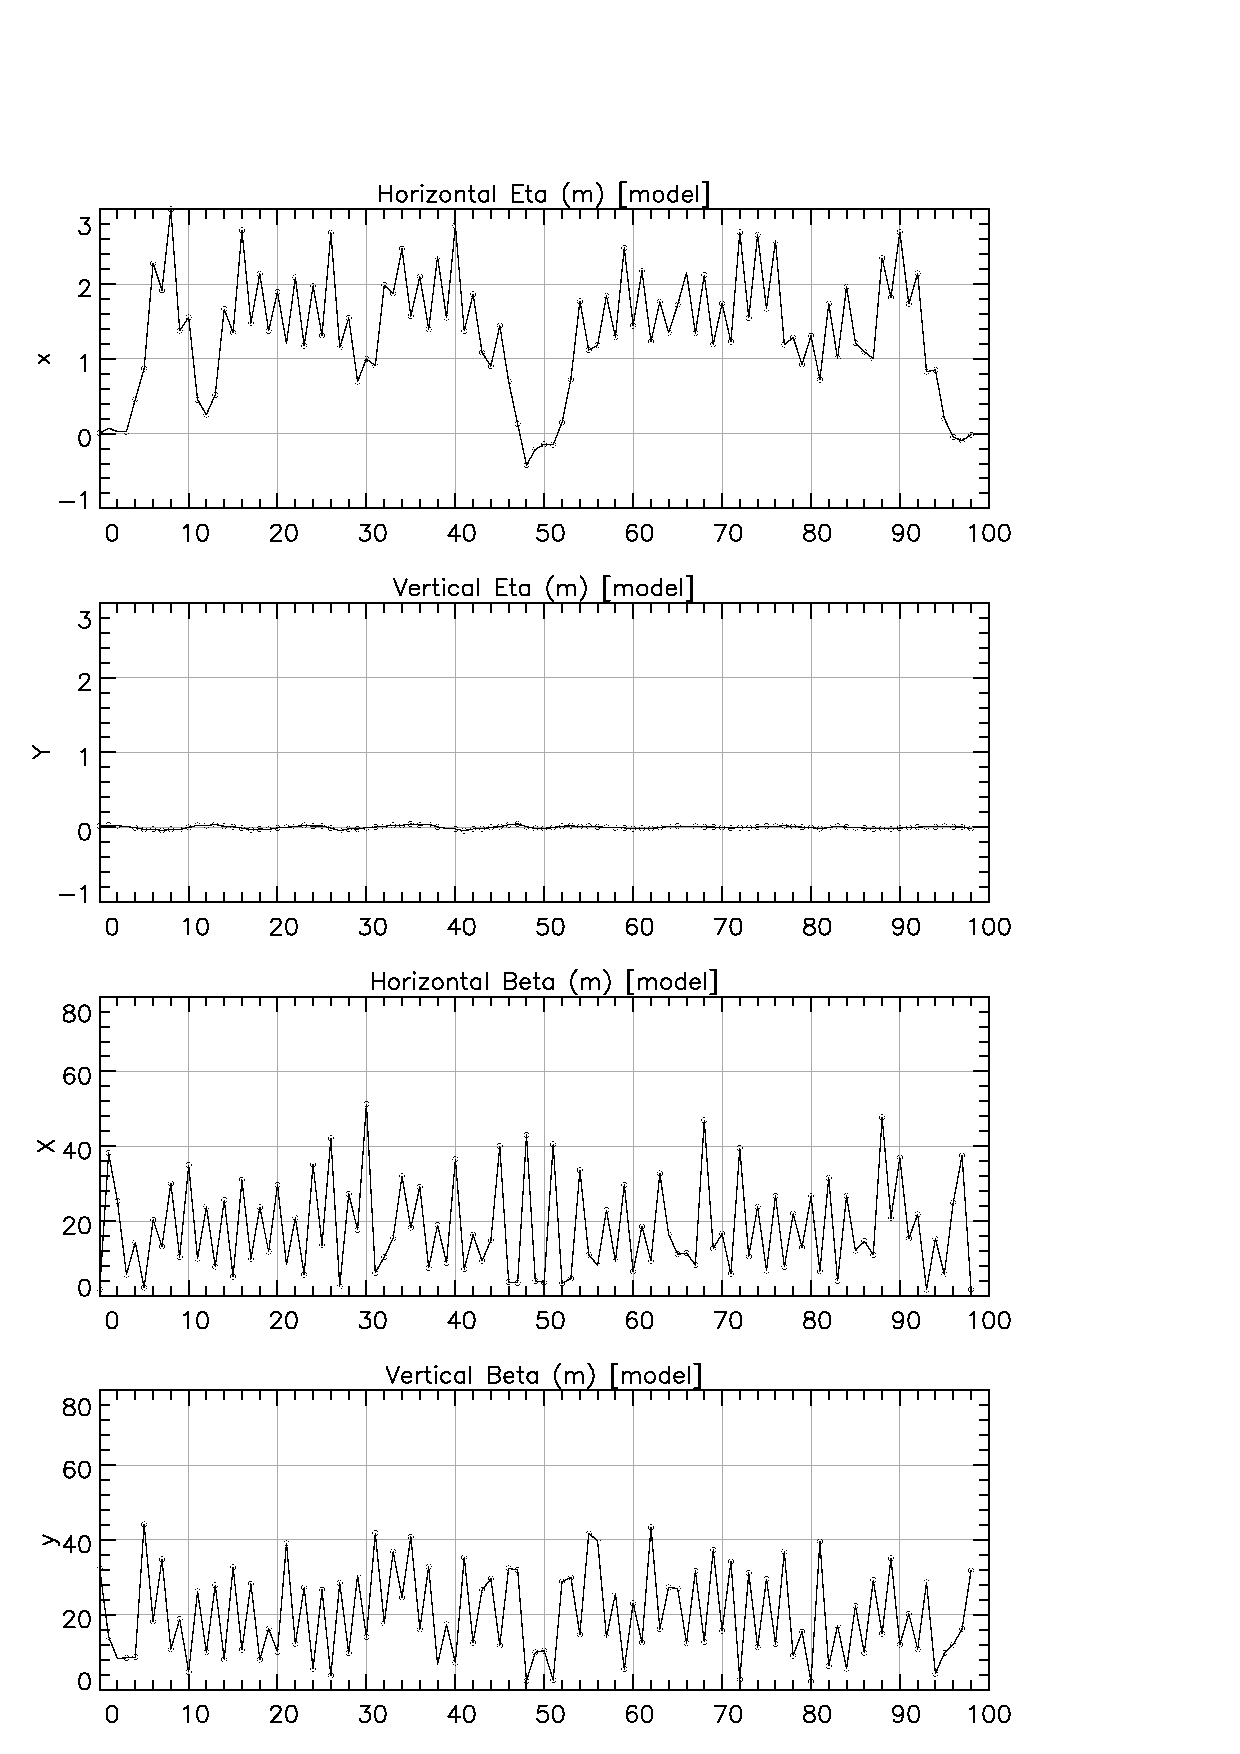
\includegraphics[width=5in]{plot_eta_beta.psfig}
  \caption{Plotting dispersion and beta function}
  \label{f:plot_eta_beta}
\end{figure}

\begin{figure}
  \centering
  \includegraphics[width=5in]{plot_coupling_no_IR.psfig}
  \caption{Zooming in on the residual coupling outside the IR.}
  \label{f:plot_coupling_no_IR}
\end{figure}

%----------------------------------------------------------------
\subsection{The \cmd{Show} Command}

Anything in the super-universe can be displayed using the \cmd{show} command. To
get a list of the data elements currently defined in \tao type
\index{Commands!show}
\begin{example}
  show data
\end{example}
the output should look like:
\begin{example}
                                                              Bounds
     d2\_Name                       Ix  d1\_Name              Lower  Upper
     orbit
                                    1  x                      0    99
                                    2  y                      0    99
     phase
                                    1  x                      0    99
                                    2  y                      0    99
     eta
                                    1  x                      0    99
                                    2  y                      0    99
     beta
                                    1  x                      0    99
                                    2  y                      0    99
     cbar
                                    1  11                     0    99
                                    2  12                     0    99
                                    3  21                     0    99
                                    4  22                     0    99
     coupling
                                    1  11b                    0    99
                                    2  12a                    0    99
                                    3  12b                    0    99
                                    4  22a                    0    99

\end{example}
There are 6 data types defined in the initialization file. The fifth
and sixth are closely related. See Part II for an explanation of the
two coupling data types.  For the first four data types there are two
data dimensions defined corresponding to the horizontal and vertical
planes. Coupling is parameterized by a 2x2 matrix so there are four
``dimensions'' for these two data types. the ``Bounds'' columns refer
to the lower and upper indexes on the datums. there are 100 BPMs in
CESR so there are 100 data points.

To see the data values for the horizontal beta function for \cesr BPMs
1 through 50 type
\begin{example}
  show data beta:x 1:50
\end{example}
Since we haven't changed any elements in the lattice yet the model
values equal the design values. Also note that \vn{beta:x} is actually
the a-mode betatron function. In regions with little or no coupling,
the a-mode is almost completely in the horizontal plane.

A significant point: The convention in \bmad is to label the twiss
parameters as \vn{x} and \vn{y} but they are actually the \vn{a} and
\vn{b} normal modes. So in regions of strong coupling \vn{beta:x} does
not correspond to \vn{orbit:x} which is always in the true horizontal
lab frame.  However, if you wish, you can re-label your twiss data
planes as \vn{a} and \vn{b}.  Section~\ref{c:init} shows you how to do
this. Keep in mind that lattice twiss parameters are defined
\textit{only for uncoupled betatron motion} so this is all that is
provided as data types for single particle tracking.  However, true
lab-frame \vn{x} and \vn{y} twiss parameters can be defined for a
distribution of particles so for particle or macroparticle beam
tracking true lab-frame \vn{x} and \vn{y} twiss parameters can be
calculated and are provided as data types for those tracking
types. See the \bmad manual for how to convert from normal mode
coordinates to lab-frame coordinates.

This tutorial uses single particle tracking and the twiss parameters
are found about the orbit of the tracked particle. there are two other
tracking types: particle beam and macroparticle beam tracking. these
tracking types will not be explored in this tutorial.

You can also view variables by typing
\begin{example}
  show var
\end{example}
To view the quadrupole k1 values for \cesr quadrupoles 5  and 20 through 30 type
\begin{example}
  sho var quad\_k1 5 20:30
\end{example}
Again, since we haven't changed any quadrupoles the model values are
all at their design values.

You can also see the details of a particular lattice element. To view
the details for quadrupole Q05W type
\begin{example}
  sho ele Q05W
\end{example}

\vn{show var} and \vn{show ele} show two completely different types of
structures in \tao. Elements are the actual lattice elements as known
to \bmad.  Variables are native \tao structures that act kind of like
\bmad \textit{overlays} and only indirectly control the lattice
elements.

A list of lattice elements between two elements can be shown by typing 
\begin{example}
  sho lattice 0:20
\end{example}
This will show a list of all the lattice elements between and including elements
0 and 20. Twiss parameters and orbit information at each element is also
provided.

Anything printed to the display using the \vn{show} command can also be printed
to a file by typing
\begin{example}
  show write <what_to_show>
\end{example}
\index{Commands!show}

A list of all intrinsic \vn{tao} commands can be found by typing
\index{Commands!help}
\begin{example}
  help
\end{example}
This will not list any custom commands. Detailed help on any individual command
can be found with
\begin{example}
  help <command\_name>
\end{example}
where \vn{<command_name>} is the command you want help with.

%----------------------------------------------------------------
%----------------------------------------------------------------
\section{Modifying the Lattice}
\label{s:modify_lattice}

\subsection{Changing a Variable}
\label{ss:change_variable}

Let's change a variable and see what happens to the lattice. We are going to
change a quadrupole strength so we should plot the change in beta and phase.
Type the following (everything after the `!' are just comments and can be
omitted):
\begin{example}
  x-axis all index        ! let the data index be the x-axis
  place top beta          ! plot Beta data on top plot
  place bottom phase      ! plot phase data on bottom plot
  plot all model - design ! plot the difference between model and design data
  scale                   ! scale all plots
\end{example}

The k1 value can be increased by 0.01 units for quadrupole Q05W by typing
\index{Commands!change}
\begin{example}
  change var quad\_k1 5 0.01
  scale
\end{example}
Note the information returned on the command line after the command and the relative changes in
beta and phase in the plot window. This is a vertically focusing quadrupole so
the vertical beta and phase is affected more than the horizontal. The \cmd{0.01}
at the end of the command tells \tao to change this variable by 0.01 units. If
you want to set a variable to a particular value then use a ``@'' before the
value. So, to change this quadrupole k1 to -0.348 type
\begin{example}
  change var quad\_k1 5 @-0.348
\end{example}

\subsection{Putting things back where you found them}
\label{ss:put_it_back}

Let's put this quadrupole back where we found it. We can also modify the quadrupole
by modifying the lattice element directly by typing
\begin{example}
  change ele Q05W k1 d0.0
\end{example}
By modifying the element directly with the \cmd{change ele} command
you can modify almost any attribute of the element listed in the
output of \cmd{show ele Q05W}.  The ``d'' before the value is used to
set the variable relative to the design value.
\index{Commands!change}

If you've changed the lattice around a lot using variables, a great way to set
all variables back to their design values is to type
\index{Commands!set}
\begin{example}
  set var all model = design
\end{example}
This only works if you just changed variables. If you changed any elements
directly with the \cmd{change ele} command then this will not work. To set
every attribute of every element back to the design type
\begin{example}
  set lattice model = design
\end{example}
Note that this will also recalculate the data and variable values
associated with the the model lattice to reflect the change so all the
bookkeeping is done for you.


%----------------------------------------------------------------
%----------------------------------------------------------------
\section{Running the Optimizer}\index{Optimization!running the optimizer}
\label{s:optimizer}

\index{lm!optimizer}\index{de!optimizer}
There are two non-linear optimizers included with \tao: Levenburg -
Marquardt, referred to as `\vn{lm}', and Differential Evolution, or
`\vn{de}'. This example will use the Levenburg - Marquardt optimizer
which first uses steepest decent to zero in on the region containing
the minimum then uses the inverse-Hessian to converge on the
minimum. See Numerical Recipes in Fortran (or C or C++) for a detailed
explanation. There's no need to know the details in order to use
either optimizer. Once you set up the problem \tao has the proper
wrapper routines to do the optimization. Of course, you are not
limited to using the included optimizers. Custom analysis can be done
using custom routines but these two optimizers have been integrated
`out of the box' with the \tao data and variable structures to make
quick optimization possible.

Basically, the `\vn{lm}' is typically faster since it uses a Jacobian
or ``dmerit'' matrix to find the data derivatives versus each variable
before starting the optimization process.  However it assumes the
second derivative is fairly smooth, so for very complex function
spaces the `\vn{de}' may work better. But because `\vn{lm}' typically
converges much faster (for functions it can handle) it is recommended
to try this one first and only use `\vn{de}' if it fails.

\subsection{Fix a Messed Up lattice}
\label{ss:fix_it}

Let's mess the lattice up a little and see if the optimizer can
``fix'' the lattice. First transfer the ``correct'' or \vn{design}
lattice to the \vn{meas} data area.
\begin{example}
  set data all meas = design
\end{example}
Now mess up the lattice a bit. We'll be messing with quadrupoles so
plot beta and phase.
\begin{example}
  place top beta
  place bottom phase
  plot all meas - model
  change var quad\_k1 10 0.001
  change var quad\_k1 21 -0.001
  change var quad\_k1 67 -0.005
  scale
\end{example}
The lattice is now sufficiently screwed up.

Now specify what variables and data to use in the optimization. First type
\begin{example}
  show top10
\end{example}
to see what data is effecting the merit function the most. The merit function is
defined by
\Begineq
  {\cal M} \equiv \sum_{i} w_i \,
    \bigl[ \data_\model(i) -  \data_\meas(i) \bigr]^2 + 
  \sum_{j} w_j \,
    \bigl[ \var_\model(j) - \var_\meas(j) \bigr]^2
  \label{eq:merit}
\Endeq
where $w_{i}$ and $w_{j}$ are the weights given to each component.
The optimizer tries to minimize the merit function by changing the model to look
like the measured data. From the \vn{top10} output we see that the beta function is effecting 
the merit function the most. Since we
are looking at beta and phase let's only use that data in the optimization.
\begin{example}
  veto data all
  use  data beta all
  use  data phase all
\end{example}
We also know that we need to change quadrupoles to correct the lattice.
\begin{example}
  veto var all         ! veto all the data
  restore var quad\_k1 all ! restore just the quad\_k1 data
\end{example}
Note that we need to specify what data and variables we will be using beforehand in the
initialization files. This is already taken care of in the demo initialization
files. You can view these files to see how the data and variables were
initialized. Raw lattice elements cannot be used by the included optimizer but
there is no such restriction on custom optimizers.

Now let's see if we have the optimizer set up correctly.
\begin{example}
  sho optimizer
\end{example}
Whoops! we want to use the Levenburg - Marquardt optimizer so
\begin{example}
  set global optimizer = lm
  sho opt
\end{example}
The second command is short-hand. Most \tao commands can be shortened to the
least number of characters needed to distinguish the command from all others.

Now we're ready to run the optimizer or ``fit'' the model to the `measured' data.
\begin{example}
  run
\end{example}
You see the optimizer going through its cycles and it did it! The model is now
``fitted.'' We can see what changes where done to the quadrupoles by typing
\begin{example}
  sho var quad\_k1
\end{example}
The optimizer came very close to finding the ``design'' lattice. However, it
changed more quadrupoles than just 10, 21 and 67. This isn't surprising. The
optimizer finds the minimum of the merit function and there are potentially many
minimums, or degeneracies.  It does it's best not to get stuck in a local
minimum and as we can see by the plotted data, the minimum found is very close
-- virtually identical -- to the design lattice optics.  A good hint as to what
variables will be adjusted is the output of \cmd{show top10}.  The top 3
derivatives were not the quadrupoles we adjusted. Nevertheless, the final result
was a darn near perfect match!

\subsection{Now Not Using all of the Variables}
\label{ss:fix_it_not_all}

Alternatively, we could have used only a subsection of the quadrupoles. Say we
know approximately which quadrupoles should be adjusted. We can then specify these
variables ranges.
\begin{example}
  change var quad\_k1 10 0.001
  change var quad\_k1 21 -0.001
  change var quad\_k1 67 -0.005
  scale
  use var quad\_k1 8:12 20:25 65:70
  run
  sho var quad\_k1 8:12 20:25 65:70
\end{example}
Different quadrupoles than the ones we initially changed were still adjusted
by the optimizer. The end result is again very close to the design lattice.

\subsection{Lattice Design}
\label{ss:lattice_design}

You may wish to constrain beam parameters instead of ``fitting'' to data. For
example, you could want the beta function not to exceed a value in a certain
part of the machine. \tao will also perform this type of optimization.

\fbox{this subsection is yet to be completed!} 

%----------------------------------------------------------------
%----------------------------------------------------------------
\section{Single Mode}\index{Single Mode}
\label{s:single_mode}

Single mode utilizes a simple single character interface to the \tao model
lattice.  By simply typing single predefined characters the specified element
parameter will be changed by a certain amount. This allows the user to quickly
converge on a neighborhood around the minimum of a multidimensional non-linear
function space. However, finding the exact minimum can be difficult to do by
hand. Once the neighborhood is found the optimizer can be used to narrow in on
the optimum configuration without requiring it to run all around the parameter
space, which is very inefficient and time consuming for complex parameter
spaces.

\fbox{this section is yet to be completed!} 

%----------------------------------------------------------------
%----------------------------------------------------------------
\section{Where to go from here}
\label{s:where_to_go}

You now have an understanding of the basic abilities of \tao. After this
tutorial, Part II of the \tao Manual should be legible and useful.
The Reference Guide will provide the details of everything mentioned in this tutorial. 
It goes into detail of setting up your own initialization
files and how to use the optimizer. It also includes a complete command
reference with command syntax.

However, you're not yet ready to customize \tao, but this is where the true versatility
of \tao lies. So, onward to the next section and learn how to write your
own custom routines to perform whatever accelerator calculations that strikes your
fancy!

%----------------------------------------------------------------
%----------------------------------------------------------------
%----------------------------------------------------------------
%----------------------------------------------------------------
\chapter{Customizing Tao}\index{Customizing}
\label{c:custom_tao}

%----------------------------------------------------------------
\section{It's all a matter of Hooks}\index{Customizing!Hooks}

The golden rule when extending \tao is that you are only allowed to replace
routines or redefine structures that have the name ``hook'' in them.  If you
have the source code then it's within your power to modify any routine in \tao
as much as you like. However, as time goes by, and revisions are made to the
\tao routines to extend the usefulness of \tao and to eliminate bugs, only
modifying the ``hook'' routines will ensure that custom changes will have a
minimum impact on the specialized routines that will be written by various
people. 

\tao is written in Fortran 95 and a knowledge of Fortran is required. However,
if you know C then Fortran can be learned in a coupled of days. Because of the
interoperability between C and Fortran once the wrapper routines are written to
interface with \tao the rest of your coding can, in principle all be done in C.

\tao relies on extensive use of pointers and logical flags. However, all of the
structures you will need to use are contained in the \vn{tao_struct.f90}
module. This module is heavily documented and provides all the information
needed to use the intrinsic \tao structures on your customizations. It is also a
very good idea to have a copy of \vn{bmad_struct.f90} handy as this contains
most of the structures used by \bmad.

%----------------------------------------------------------------
\section{Compiling your custom Tao}
\index{Customizing!Compiling}

The \tao libraries can be compiled without compiling an executable. Here is
where this comes in handy. Since the standard \tao subroutines have already been
made into libraries, all you need to do is compile and link your custom
routines with the standard \tao subroutines into an executable.

There are 11 ``hook'' files located in the \cmd{ROOT/tao/hook} directory. These are
the files you can customize. There are two options here. 
\begin{enumerate}
  \item Change the files directly in \cmd{ROOT/tao/hook}, adding any extra
    files you may need, then recompile from the \cmd{ROOT/tao} directory with
  \cmd{gmake -f M.tao}.  \label{cust_option_one}
  \item Copy the hook files to a separate directory say \cmd{ROOT/my_tao},
    adding any extra files you may need, then write a Makefile to compile and link these
    routines to the main \tao library. \label{cust_option_two}
\end{enumerate}
Option~\ref{cust_option_two} is HIGHLY recommended because it keeps the \tao
distribution tree undisturbed and reserves the possibility to create multiple
custom \tao programs using the same vanilla \tao library. This option is used in
the following example.

%----------------------------------------------------------------
\section{An Example}\index{Customizing!Example}

As an example let's include a new data type called \vn{particle_emittance}. This
will be the non-normalized x and y emittance as found from the Courant-Snyder
invariant. This data type will behave just like any other data type (i.e.
\vn{orbit}, \vn{phase} etc...). First, we should copy all the hook files to a
separate directory, call it \cmd{ROOT/my_tao}. Also include the main program file
from the \cmd{ROOT/tao/program} directory.  (replace \vn{ROOT} with whatever top
directory you placed the \vn{tao} directory.)
\begin{example}
  mkdir ROOT/my_tao
  cp ROOT/tao/hook/*.f90 ROOT/my_tao
  cp ROOT/tao/program/tao_cl.f90 ROOT/my_tao/my_tao_cl.f90
\end{example}
Next we need a Makefile. The \cmd{ROOT/tao/M.tao} 
Makefile is a great starting point.
\begin{example}
  cp ROOT/tao/M.tao ROOT/my_tao/Makefile
\end{example}
Now change the following lines in your Makefile
\begin{example}
  LIB\_SRC\_DIRS := ./code ./hook
  OBJ\_SRC\_DIRS := ./program
\end{example}
to
\begin{example}
  LIB\_SRC\_DIRS :=
  OBJ\_SRC\_DIRS := ./
\end{example}
This Makefile will tell gmake to use the tao library that has already been created (from 
\cmd{../tao/code} but the actual library is located at \cmd{../lib/libtao.a})
 and then to compile
all of the hook files, including the main program file (\cmd{my_tao_cl.f90})
into object files (everything in \cmd{./}, the current directory).  Routines and
declarations in object files always override similarly named code in the \tao
libraries so this allows for your local hook files to override the dummy hook
files in the \tao library. The only downside to this method is it clutters your
\cmd{my_tao} directory with object files. You can always remove these object files
with \cmd{gmake clean}.

There are two more lines to alter. change
\begin{example}
  MAIN\_FILE :=
\end{example}
to
\begin{example}
  MAIN\_FILE := ./my\_tao_cl.f90
\end{example}
and finally,
\begin{example}
  MAKEFILE := M.tao
\end{example}
to
\begin{example}
  #MAKEFILE := M.tao !using default name for Makefile
\end{example}
Notice that this line is just being commented out with a `\#'. You are now ready
to make your customizations to the hook routines.

This example will only require the modification of one file:
\vn{tao_hook_load_data_array.f90}. The formula for single particle emittance is
\Begineq
  \epsilon = \gamma x^{2} + 2 \alpha x x' + \beta x'^{2}
  \label{e:emittance}
\Endeq
Place the following code in \vn{tao_hook_load_data_array.f90} in the
\cmd{case select} construct (also add the necessary type declarations)
\begin{verbatim}
  case ('particle_emittance:x') 

    datum_value =  ( ele%x%gamma * orb(ix1)%vec(1)**2 + &
		     2 * ele%x%alpha * orb(ix1)%vec(1) * orb(ix1)%vec(2) + &
		     ele%x%beta * orb(ix1)%vec(2)**2)
    
  case ('particle_emittance:y')

    datum_value = ( ele%y%gamma * orb(ix1)%vec(3)**2 + &
		     2 * ele%y%alpha * orb(ix1)%vec(3) * orb(ix1)%vec(4) + &
		     ele%y%beta * orb(ix1)%vec(4)**2)
\end{verbatim}
This defines what is to be calculated for each \vn{particle_emittance} datum.
There are two transverse coordinates, so two definitions need to be made, one for
each dimension.

Now you just need to declare the data types in the \cmd{tao.init} and
\cmd{tao_plot.init} files. For the sake of this example, modify the
initialization files used for this tutorial.
\begin{example}
  cp ROOT/tao/program/*.init ROOT/my_tao
  cp ROOT/tao/program/*.lat ROOT/my_tao
\end{example}

In \cmd{ROOT/my_tao/tao.init} add the following lines to the data
declarations section
\begin{example}
  &tao_d2_data
    d2_data%name = "particle_emittance" 
    universe = 0 
    n_d1_data = 2
  /

  &tao_d1_data
    ix_d1_data = 1
    d1_data%name = "x"  
    default_weight = 1
    ix_min_data = 0 
    ix_max_data = 99  
    data(0)%name = "SAME: orbit:x"
    data(0)%ele_name = "SAME: orbit:x"
  /

  &tao_d1_data
    ix_d1_data = 2
    d1_data%name = "y"  
    default_weight = 1
    ix_min_data = 0 
    ix_max_data = 99  
    data(0)%name = "SAME: orbit:x"
    data(0)%ele_name = "SAME: orbit:x"
  /
\end{example}
and increase \vn{n_d2_data_max} to 7 in the \vn{tao_params} declaration.

In \cmd{ROOT/my_tao/tao_plot.init} add the following lines to the end
of the file
\begin{example}
  &tao_template_plot
    plot%name = 'particle_emittance'
    plot%x%min =   0
    plot%x%max = 100
    plot%x%major_div = 10
    plot%x%label = ' '
    plot%x_axis_type = 'index'
    plot%n_graph = 2
  /
  
  &tao_template_graph
    graph%name = 'x'
    graph_index = 1
    graph%box = 1, 2, 1, 2
    graph%title = 'Horizontal Emittance (microns)'
    graph%margin =  0.15, 0.06, 0.12, 0.12, '%BOX'
    graph%y%label = 'x'
    graph%y%max =  15
    graph%y%min =  0.0
    graph%y%major_div = 4
    graph%n_curve = 1
    curve(1)%data_source = 'data_array'
    curve(1)%data_type   = 'particle_emittance:x'
    curve(1)%units_factor = 1e6 !convert from meters to microns
  /

  &tao_template_graph
    graph%name = 'y'
    graph_index = 2
    graph%box = 1, 1, 1, 2
    graph%title = 'Vertical Emittance (microns)'
    graph%margin =  0.15, 0.06, 0.12, 0.12, '%BOX'
    graph%y%label = 'Y'
    graph%y%max =  15
    graph%y%min =  0.0
    graph%y%major_div = 4
    graph%n_curve = 1
    curve(1)%data_source = 'data_array'
    curve(1)%data_type = 'particle_emittance:y'
    curve(1)%units_factor = 1e6 !convert from meters to microns
  /
\end{example}
These namelists are described in detail in Chapter~\ref{c:init}.

We are now ready to compile and then run the program. The \tao library should have
already been created (in section~\ref{s:get_and_compile}) so all you need to do is
\begin{example}
  cd ROOT/my_tao
  gmake
  ../bin/my_tao_cl
\end{example}
Notice that the name of the custom \tao program is \cmd{my_tao_cl}. If you run 
`\cmd{../bin/tao}' then you will run ``vanilla'' \tao.

After your custom \tao initializes type
\begin{example}
  place bottom particle_emittance
  scale
\end{example}
Your plot should look like Figure~\ref{f:plot_emittance}.

The emittance (as calculated) is not constant. This is due to dispersion and
coupling throughout the ring. \bmad provides a routine to find the particle
emittance from the twiss parameters that includes dispersion and coupling called
\vn{orbit_amplitude_calc}.

\begin{figure}
  \centering
  \includegraphics[width=5in]{plot_emittance.psfig}
  \caption{Custom data type: non-normalized emittance}
  \label{f:plot_emittance}
\end{figure}

\Section{Other Customizations}

The above example just illustrates one of the customizations you can perform on \tao.
Part III, Programmer's Guide lays out all of the hook files and provides pointers
for various customizations.

